\scanpage{8}
Si $\unsure{\mathscr{T}|\mathcal{T}}$ est le groupe des racines de l'unité dans $\mathbb{C}$, \deleted{donc} i.e. le ss-gpe de
torsion de $\mathbb{C}^{\unsure{\times|*}}$, qui est isomorphe à
$\mathbb{Q}/\mathbb{Z}$, \deleted{donc dans $\mathscr{T}$ il y a un unique \unsure{élém|élément} d'ordre 2, savoir $-1$, engendre l'unique ss-gpe cyclique d'ordre 2, $\{\pm1\}\subset\mathscr{T}$}
donc $\pm1$ opère sur
$\mathscr{T}$ (écrit additivement pour les besoins de la
cause) et \deleted{$\unsure{\mathscr{T}/\pm1|\mathscr{T}/\{\pm1\}}$} l'ens des classes
d'isom de \unsure{polygones|polygônes} réguliers sur $\mathbb R$
est en corr. biunivoque canonique
avec $\bigl(\mathscr{T}/\{\pm1\}\mathbin{\backslash}\{0_{\mathscr{T}}\}\bigr)$ où $0_{\mathscr{T}}$ est l'image
dans le quotient $\mathscr{T}/\{\pm1\}$ de l'élt. nul de $\mathscr{T}$.

On a pour quatre pts consécutifs $s_i,s_{i+1},s_{i+2},s_{i+3}$
\[
(s_{i+3}-s_i)=\deleted{\unsure{\zeta|(+}}r(s_{i+2}-s_{i+1})
\]
\figure{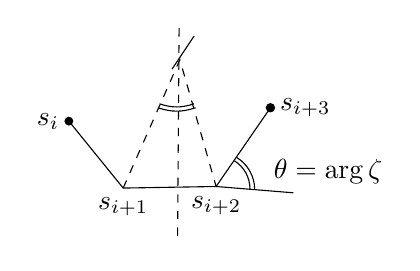
\begin{tikzpicture}[x=1cm,y=1cm]
\coordinate (s0) at (0,.91); \coordinate (s1) at (.69,.06);
\coordinate (s2) at (1.87,.08); \coordinate (s3) at (2.56,1.08);
\coordinate (t) at (1.41,1.69);
\draw (s0)--(s1)--(s2)--(s3); \draw (s2)--(2.85,0);
\draw[dashed] (s1)--(t)--(s2); \draw[dashed] (1.40,2.09)--(1.38,-.63);
\draw (1.31,1.57)--(1.59,1.99);
\draw (1.15,1.13) to[bend right=18] (1.59,1.13);
\draw (1.13,1.08) to[bend right=18] (1.61,1.08);
\draw (2.36,.04) arc[start angle=0,end angle=58,radius=.48];
\draw (2.30,.05) arc[start angle=0,end angle=58,radius=.42];
\fill (s0) circle (1.6pt) node[left] {$s_i$};
\node[below] at (s1) {$s_{i+1}$}; \node[below] at (s2) {$s_{i+2}$};
\fill (s3) circle (1.7pt) node[right] {$s_{i+3}$};
\node[right] at (2.48,.27) {$\theta=\arg\zeta$};
\end{tikzpicture}}
où $r$ est un nb \uline{réel} qui ne dépend
que de $\zeta$ (pas de $i$) en fait
\[
r=1+\underbrace{(\zeta+\zeta^{-1})}_{2\cos\arg\zeta}
\]
En effet,
\[
\frac{\zeta^{i+3}-\zeta^i}{\zeta^{i+2}-\zeta^{i+1}}\deleted{\unsure{=}}=
\frac{\zeta^3-1}{\zeta^2-\zeta}=
\frac{\zeta^2+\zeta+1}{\deleted{\unsure{\zeta^2-}}\zeta}=1+(\zeta+\zeta^{-1})
\]
% archive sheet number: 7

